\documentclass[preprint,12pt]{elsarticle}

\usepackage{graphicx}
\usepackage{booktabs}
\usepackage{amsmath,amssymb}
\usepackage{multirow}
\usepackage{float}
\usepackage{tabularx}
\usepackage{makecell}
\usepackage[hidelinks]{hyperref}
\usepackage{url}
\urlstyle{same}

\journal{Applied Energy}

\newcolumntype{Y}{>{\centering\arraybackslash}X}
\emergencystretch=2em

\begin{document}

\begin{frontmatter}

\title{Design-actionable cost--resilience thresholds for islanded
battery--hydrogen microgrids: component drivers, diesel-support robustness,
and dynamic feasibility}

\author{Jaewon Lee}
\address{National Institute of Green Technology, Republic of Korea}

\begin{abstract}
Islanded and remote microgrids increasingly weigh battery--hydrogen storage
against diesel-backed batteries, yet the conditions under which hydrogen is
actually justified remain imprecisely defined. The cost, resilience, and
frequency-stability dimensions of this choice have each been studied, but
usually in separate analyses and for a single optimised design per
technology---leaving open which design levers move the economic threshold,
whether the resilience advantage is intrinsic to hydrogen or a by-product of its
sizing, and how robust the verdict is to the assumed level of diesel support.
Using an 8760-h cost-optimal dispatch model driven by real NASA POWER weather
for a representative Philippine off-grid island, we bring these dimensions
together into a single, design-actionable, multi-axis comparison of a
battery--hydrogen portfolio against a PV--diesel--battery portfolio. We find an
economic crossover at a delivered diesel cost of 378~USD/MWh. A component-level
decomposition shows the frontier is governed primarily by photovoltaic capital
cost---because the hydrogen portfolio is intrinsically PV-intensive---rather than
by electrolyser or fuel-cell efficiency. A matched-backbone comparison
demonstrates that the resilience advantage is structural: on an identical
PV--battery spine, the diesel--battery system cannot bridge the worst-case
48-hour outage---it sheds critical load and provides no guaranteed uninterrupted
service (worst-case critical-load survivability 0.98)---whereas the
battery--hydrogen system sustains the full 48 hours, owing to long-duration
hydrogen storage. A graded diesel-support stress
test shows that any derating below roughly 50\%, any fuel budget below about 12
hours, or any delivery delay collapses the diesel--battery worst-case
survivability, and a reduced-order frequency screen confirms that this weakness
extends to the dynamic layer during the diesel-trip grid-forming handover.
Battery--hydrogen is therefore defensible whenever delivered diesel is costly or
diesel support is degradable---precisely the conditions that characterise
remote-island contingencies.
\end{abstract}

\begin{keyword}
islanded microgrid \sep green hydrogen \sep long-duration storage \sep
resilience \sep cost threshold \sep grid-forming inverter \sep frequency stability
\end{keyword}

\end{frontmatter}

%=====================================================================
\section{Introduction}
\label{sec:intro}

Remote and islanded power systems serve a large and growing share of the world's
un- and under-electrified population and remain overwhelmingly dependent on
diesel generation \cite{hirsch_2018_microgrids_review,akinyele_2018_remote_microgrid_challenges}.
In archipelagic countries such as the Philippines, hundreds of small island grids
rely on imported diesel whose delivered cost is inflated by maritime logistics and
is highly volatile, while the same islands face frequent typhoon-driven
disruptions that can sever fuel resupply for days
\cite{ocon_bertheau_2019_philippines_diesel_pvbatt,castro_2022_634_islands_hres,castro_2023_busuanga_resilience}.
These systems therefore sit at the intersection of two pressures that are usually
studied separately: decarbonisation, which favours displacing diesel with solar
and storage, and resilience, which requires riding through multi-day
contingencies when external supply fails.

Battery--hydrogen hybrids are increasingly proposed to address both pressures,
pairing short-duration batteries with a long-duration hydrogen store---electrolyser,
tank, and fuel cell---that can in principle sustain critical load through extended
outages without fuel deliveries
\cite{alzahrani_2022_hydrogen_microgrid_review,van_2023_hydrogen_microgrid_review,staadecker_2024_ldes_value}.
Hydrogen subsystems are, however, capital-intensive and round-trip inefficient, so
whether they are justified over a conventional PV--diesel--battery design depends
on site-specific economics and on how severe and how diesel-dependent the
resilience requirement is. Establishing the \emph{thresholds} that separate the
two designs---and, crucially, identifying which design levers move those
thresholds---is what makes such an analysis actionable for planners rather than
merely descriptive.

A substantial literature optimises the sizing and dispatch of hybrid
renewable--storage microgrids
\cite{pascasio_2021_philippines_pv_wind,castro_2024_208_islands_transition,meschede2019transferability},
and a growing body of work examines hydrogen specifically in island and off-grid
contexts \cite{tatti_2024_hydrogen_offgrid_case,alharbi2025comparative,qi_2025_h2_battery_dispatch}.
Resilience-oriented studies introduce metrics such as expected energy not served
and critical-load survivability and couple them to outage scenarios
\cite{marqusee2021resilience,gao_2016_critical_load_restoration,raoufi_2020_power_resilience_metrics,amiri_2024_resilience_framework}.
In parallel, the power-electronics community has established that
inverter-dominated islanded grids require explicit grid-forming sources and that
frequency stability---rate of change of frequency (RoCoF) and frequency
nadir---becomes a binding design concern as synchronous inertia disappears
\cite{liu2016comparison,shahgholian2025droop,chamorro2020innovative,olasoji2024review}.

Each of these dimensions has been studied, often in depth. What remains uncommon
is to bring them together into a single, decision-actionable comparison. In
particular: (i) economic thresholds are usually reported for one optimised design
rather than attributed to the specific component costs that move them; (ii)
competing portfolios are compared as separately optimised designs, which conflates
the storage technology with the sizing it induces---controlled comparisons on a
common PV--battery backbone, which would isolate the technology's own
contribution, are rare; (iii) the level of diesel support during an outage is
fixed at one or a few scenarios rather than swept as a continuous robustness
boundary that locates where a diesel--battery system matches hydrogen; and (iv)
the economic, resilience, and frequency-stability verdicts are typically
established in separate studies, so their mutual consistency for a given design is
seldom verified
\cite{huang_2023_economic_resilient_h2_microgrid,shahbazbegian_2023_resilience_p2h,sharifpour_2023_hydrogen_extreme_events,sepulveda_2021_ldes_design_space,rosales_asensio_2022_critical_customers,mishra2023microgrid,bertheau2018resilient}.

This paper addresses these gaps with a unified, design-actionable threshold
analysis of a battery--hydrogen versus a PV--diesel--battery portfolio, built on
an 8760-h cost-optimal dispatch model driven by real NASA POWER weather (calendar
year 2025, central Visayas) for a representative Philippine off-grid island, with
a calibrated representative load profile. The contributions are: (i) a fine
cost--resilience frontier locating the economic crossover and its sensitivity to
hydrogen capital cost; (ii) a component-level decomposition identifying which cost
and efficiency parameters most move that frontier; (iii) a matched-backbone
comparison---the methodological centrepiece---that places both portfolios on a
common PV--battery spine to isolate the contribution of the flexibility technology
from sizing; (iv) a graded diesel-support stress test that treats the
diesel-availability assumption as a continuous robustness boundary across
derating, fuel-budget, and delivery-delay cases; and (v) a reduced-order
frequency-stability screen with explicit grid-forming source assignment for each
portfolio and operating mode, integrated into the same framework so the economic,
resilience, and dynamic verdicts are mutually consistent. The findings are not the
expected truism that hydrogen wins when diesel is dear, but a set of more specific
and partly counter-intuitive results: the economic crossover occurs at a delivered
diesel cost of 378~USD/MWh; the frontier is governed primarily by PV capital
cost---not hydrogen component cost or efficiency---because the hydrogen portfolio
is intrinsically PV-intensive; the resilience advantage is structural, persisting
even at a matched backbone, where the diesel--battery system cannot bridge the
worst-case 48-hour outage---sheds critical load with zero guaranteed survivable
hours---against hydrogen's full 48 hours; and this
advantage extends to the frequency-dynamic layer, where the diesel--battery system
is weakest precisely during the diesel-trip handover that also drives its
energy-resilience weakness. Together these results show that battery--hydrogen is
defensible whenever delivered diesel is costly or diesel support is degradable,
both of which characterise remote-island contingencies.

The remainder of the paper is organised as follows.
Section~\ref{sec:methods} describes the system model, cost formulation, resilience
evaluation, and the reduced-order dynamic screen; Section~\ref{sec:case} gives the
case study and assumptions. Section~\ref{sec:results} presents the threshold
frontier and its component drivers, the matched-backbone comparison, the
diesel-support robustness analysis, and the frequency-stability screen.
Section~\ref{sec:disc} discusses design implications and limitations, and
Section~\ref{sec:concl} concludes.

%=====================================================================
\section{Methods}
\label{sec:methods}

We compare three fixed-architecture portfolios for an islanded microgrid: a
PV--battery system (battery-only), a PV--diesel--battery system
(diesel-battery), and a PV--battery--hydrogen system
(battery-hydrogen). For each portfolio we (i) solve an 8760-h
cost-optimal dispatch, (ii) accumulate an annualised total cost, (iii) evaluate
critical-load resilience over a stochastic outage set, and (iv) screen
primary-frequency dynamics with a reduced-order model. Sections~\ref{sub:thresh}
and \ref{sub:robust} define the cost--resilience threshold, the matched-backbone
construction, and the diesel-support robustness sweep that the Results build on.

\subsection{Sets, variables, and parameters}
Let $t \in \mathcal{T}=\{1,\dots,8760\}$ index the hours of one year, with time
step $\Delta t = 1\,\mathrm{h}$. The hourly decision variables are the used PV
power $p^{\mathrm{pv}}_t$, battery charge and discharge powers
$p^{\mathrm{ch}}_t,\,p^{\mathrm{dis}}_t$ and state of charge $e_t$, diesel power
$p^{\mathrm{dg}}_t$, fuel-cell power $p^{\mathrm{fc}}_t$, electrolyser power
$p^{\mathrm{el}}_t$, hydrogen inventory $m_t$, and unserved load $u_t$ (all
$\ge 0$). Fixed inputs are the demand $D_t$ and the available PV
$\hat{p}^{\mathrm{pv}}_t$. Installed sizes are $\bar S^{\mathrm{pv}}$, battery
power $\bar S^{\mathrm{bp}}$ and energy $\bar S^{\mathrm{be}}$,
$\bar S^{\mathrm{dg}}$, $\bar S^{\mathrm{fc}}$, $\bar S^{\mathrm{el}}$, and tank
$\bar S^{\mathrm{tk}}$ (kg). Round-trip parameters are battery charge/discharge
efficiencies $\eta^{\mathrm{ch}},\eta^{\mathrm{dis}}$, electrolyser and fuel-cell
LHV efficiencies $\eta^{\mathrm{el}},\eta^{\mathrm{fc}}$, and the hydrogen lower
heating value $\mathrm{LHV}=33.3\,\mathrm{kWh\,kg^{-1}}$. Cost parameters are
summarised in Table~\ref{tab:assumptions}.

\subsection{Optimal dispatch model}
For fixed capacities, the hourly dispatch minimises annual operating cost,
\begin{equation}
\label{eq:obj}
\begin{aligned}
\min \; \sum_{t\in\mathcal{T}} \Big[ & (c^{\mathrm{fuel}} + c^{\mathrm{co_2}}\varepsilon^{\mathrm{dg}})\,p^{\mathrm{dg}}_t + c^{\mathrm{thr}}\,(p^{\mathrm{ch}}_t + p^{\mathrm{dis}}_t) \\
& + c^{\mathrm{el}}\,p^{\mathrm{el}}_t + c^{\mathrm{fc}}\,p^{\mathrm{fc}}_t + c^{\mathrm{pen}}\,u_t \Big]\,\Delta t,
\end{aligned}
\end{equation}
where $c^{\mathrm{fuel}}$ is the delivered diesel cost (USD MWh$^{-1}$ of
electrical output), $\varepsilon^{\mathrm{dg}}=0.70$~t CO$_2$ MWh$^{-1}$ the diesel
emission factor, $c^{\mathrm{co_2}}$ the carbon price, $c^{\mathrm{thr}}=1$~USD
MWh$^{-1}$ a battery throughput (cycling) cost charged on both charge and
discharge, $c^{\mathrm{el}}=2$ and $c^{\mathrm{fc}}=4$~USD MWh$^{-1}$ small
electrolyser and fuel-cell variable-O\&M terms, and $c^{\mathrm{pen}}=10{,}000$~USD
MWh$^{-1}$ a high unserved-energy penalty that makes load-shedding a last resort
within the dispatch (a modelling device, distinct from the value of lost load used
for resilience in Section~\ref{sub:resil}). With $\Delta t=1\,\mathrm{h}$, each
hourly power term equals its energy. Subject to, for all $t$, PV allocation with
explicit curtailment $p^{\mathrm{cu}}_t$ and the system power balance,
\begin{equation}
\label{eq:pv}
p^{\mathrm{pv}}_t + p^{\mathrm{cu}}_t = \hat{p}^{\mathrm{pv}}_t = \bar S^{\mathrm{pv}}\,\gamma_t,
\end{equation}
\begin{equation}
\label{eq:bal}
p^{\mathrm{pv}}_t + p^{\mathrm{dis}}_t + p^{\mathrm{dg}}_t + p^{\mathrm{fc}}_t + u_t \;=\; D_t + p^{\mathrm{ch}}_t + p^{\mathrm{el}}_t,
\end{equation}
where $\gamma_t\in[0,1]$ is the PV capacity factor. Storage dynamics use battery
charge/discharge efficiencies $\eta^{\mathrm{ch}}=\eta^{\mathrm{dis}}=0.95$ and
hydrogen conversion coefficients
$\kappa^{\mathrm{el}}=10^{3}\eta^{\mathrm{el}}/\mathrm{LHV}=20.1$~kg MWh$^{-1}$ and
$\kappa^{\mathrm{fc}}=10^{3}/(\eta^{\mathrm{fc}}\,\mathrm{LHV})=60.0$~kg MWh$^{-1}$,
\begin{equation}
\label{eq:soc}
\begin{gathered}
e_t = e_{t-1} + \eta^{\mathrm{ch}} p^{\mathrm{ch}}_t \Delta t - \tfrac{1}{\eta^{\mathrm{dis}}} p^{\mathrm{dis}}_t \Delta t, \\
m_t = m_{t-1} + \kappa^{\mathrm{el}} p^{\mathrm{el}}_t \Delta t - \kappa^{\mathrm{fc}} p^{\mathrm{fc}}_t \Delta t,
\end{gathered}
\end{equation}
with bounds $0\le e_t\le\bar S^{\mathrm{be}}$, $0\le m_t\le\bar S^{\mathrm{tk}}$,
and rated-power limits $p^{\mathrm{ch}}_t,p^{\mathrm{dis}}_t\le\bar S^{\mathrm{bp}}$,
$p^{\mathrm{dg}}_t\le\bar S^{\mathrm{dg}}$, $p^{\mathrm{fc}}_t\le\bar S^{\mathrm{fc}}$,
$p^{\mathrm{el}}_t\le\bar S^{\mathrm{el}}$. Both stores are initialised at 50\% of
capacity and constrained to return to that level at year-end, giving an annually
self-consistent cycle. The implied hydrogen round-trip efficiency is
$\kappa^{\mathrm{el}}/\kappa^{\mathrm{fc}}=33.5\%$. The program is a linear program
solved with HiGHS; capacities enter as fixed bounds, so the diesel cost and carbon
price affect dispatch while capital costs do not.

\subsection{Cost formulation and levelised cost}
The reported annual cost adds annualised capital and fixed O\&M to the optimised
operating cost. Capital is annualised with the capital recovery factor
\begin{equation}
\label{eq:crf}
\mathrm{CRF} = \frac{i\,(1+i)^{L}}{(1+i)^{L}-1}, \qquad i=0.07,\; L=20\,\mathrm{yr} \;\Rightarrow\; \mathrm{CRF}=0.0944.
\end{equation}
With unit capital costs $c^{\mathrm{cap}}_k$ over components $k$ (PV, battery
power, battery energy, diesel, fuel cell, electrolyser, and tank), the total
overnight capital is $\mathrm{CAPEX}=\sum_k c^{\mathrm{cap}}_k \bar S_k$, and
the total annual cost is
\begin{equation}
\label{eq:ac}
\begin{aligned}
\mathrm{AC} = {} &
\underbrace{\mathrm{CRF}\cdot\mathrm{CAPEX}}_{\text{annualised CAPEX}}
+ \underbrace{\phi\cdot\mathrm{CAPEX}}_{\text{fixed O\&M}}
+ \underbrace{c^{\mathrm{fuel}}E^{\mathrm{dg}}}_{\text{fuel}} \\[2pt]
& + \underbrace{c^{\mathrm{co_2}}\varepsilon^{\mathrm{dg}} E^{\mathrm{dg}}}_{\text{carbon}}
+ \underbrace{c^{\mathrm{thr}}E^{\mathrm{thr}} + c^{\mathrm{el}}E^{\mathrm{el}} + c^{\mathrm{fc}}E^{\mathrm{fc}}}_{\text{variable O\&M}}
+ \underbrace{c^{\mathrm{pen}}E^{\mathrm{uns}}}_{\text{unserved}} ,
\end{aligned}
\end{equation}
where $\phi=0.025$ is the fixed-O\&M rate; $E^{\mathrm{dg}}=\sum_t
p^{\mathrm{dg}}_t\Delta t$ is annual diesel energy; $E^{\mathrm{thr}}$ battery
throughput; $E^{\mathrm{el}},E^{\mathrm{fc}}$ electrolyser and fuel-cell
throughput; and $E^{\mathrm{uns}}=\sum_t u_t\Delta t$ unserved energy. The
levelised cost of electricity is
$\mathrm{LCOE} = \mathrm{AC}\,/\!\sum_t (D_t-u_t)\Delta t$, i.e. annual cost
divided by annual served energy.

\subsection{Resilience evaluation}
\label{sub:resil}
Resilience is assessed on a stochastic set of islanding events. For an annual
frequency $f^{\mathrm{out}}$ and a fixed duration $\Delta^{\mathrm{out}}$, the
outage set is
\begin{equation}
\label{eq:omega}
\Omega(s) = \big\{\,\omega_j = (\tau_j,\Delta^{\mathrm{out}}) : \tau_j \sim \mathcal{U}\{1,8760\},\; j=1,\dots,f^{\mathrm{out}} \,\big\},
\end{equation}
with start hours drawn reproducibly from seed $s$. During each event the
controllable sources serve the critical load $D^{\mathrm{crit}}_t = \alpha D_t$
(critical fraction $\alpha=0.55$) from the inventory carried into the event, using
a priority dispatch (PV $\rightarrow$ battery $\rightarrow$ fuel cell $\rightarrow$
diesel, the last subject to Section~\ref{sub:robust}). For a single event $\omega$,
\begin{equation}
\label{eq:eens}
\begin{gathered}
\mathrm{EENS}_\omega = \!\!\sum_{t\in\omega}\!\big(D^{\mathrm{crit}}_t - s_t\big)\Delta t, \\[2pt]
\mathrm{CLSR}_\omega = \frac{\sum_{t\in\omega} s_t}{\sum_{t\in\omega} D^{\mathrm{crit}}_t},
\end{gathered}
\end{equation}
where $s_t$ is the critical load served in hour $t$. The survivable duration
$\Sigma_\omega$ is the number of contiguous hours from the event start before the
first unserved hour. We report the worst case over the event set
($\mathrm{CLSR}_{\min}$, $\mathrm{EENS}_{\max}$, $\Sigma_{\min}$) and---to monetise
resilience---a value of lost load $\mathrm{VOLL}=5000$~USD MWh$^{-1}$ applied to
expected EENS, giving the resilience-adjusted cost
$\mathrm{AC}^{\mathrm{res}} = \mathrm{AC} + \mathrm{VOLL}\cdot\mathbb{E}_\Omega[\mathrm{EENS}]$.
The base case uses $f^{\mathrm{out}}=4\,\mathrm{yr^{-1}}$,
$\Delta^{\mathrm{out}}=48\,\mathrm{h}$; worst-case statistics are taken over ten
seeds unless stated.

\subsection{Cost--resilience threshold and matched backbone}
\label{sub:thresh}
The economic comparison is summarised by the cost gap
$\Delta C(c^{\mathrm{fuel}},\mu) = \mathrm{AC}_{\mathrm{BH}}(\mu) - \mathrm{AC}_{\mathrm{DB}}(c^{\mathrm{fuel}})$,
where $\mu$ scales the hydrogen-subsystem capital costs (electrolyser, fuel cell,
tank). The \emph{economic crossover} $c^{\star}(\mu)$ solves
$\Delta C(c^{\star},\mu)=0$; the resilience-adjusted crossover uses
$\Delta C^{\mathrm{res}} = \Delta C + \mathrm{VOLL}\,(\mathbb{E}[\mathrm{EENS}_{\mathrm{BH}}]-\mathbb{E}[\mathrm{EENS}_{\mathrm{DB}}])$.
To separate the storage technology from the capacity it induces, the
\emph{matched-backbone} comparison assigns both portfolios a common PV size and
battery energy (battery power at an energy-to-power ratio of 6~h), differing only
in the flexibility subsystem. Comparing the two on an identical backbone isolates
the contribution of the flexibility technology to cost and resilience.

\subsection{Diesel-support robustness}
\label{sub:robust}
The base resilience case assumes diesel is unavailable during islanding. To test
the sensitivity of the verdict to this assumption, the diesel contribution within
an event is parameterised by a derating fraction $\delta\in(0,1]$, a fuel budget
$B$ (hours at rated power), and a start delay $h_{\mathrm d}$, giving an effective
deliverable power $\delta\,\bar S^{\mathrm{dg}}$ available only for
$t\ge \tau+h_{\mathrm d}$ and only while cumulative diesel energy is below
$B\,\bar S^{\mathrm{dg}}$. The cases are: D0 unavailable; D1
$\delta\in\{0.25,0.5,0.75\}$; D2 $B\in\{3,6,12,24\}\,\mathrm{h}$; D3
$h_{\mathrm d}\in\{6,12,24\}\,\mathrm{h}$; and D4 a delivered-fuel-cost shock on
the annual economics. The hydrogen portfolio carries no diesel and is the
invariant reference.

\subsection{Reduced-order frequency-stability screen}
\label{sub:freq}
To confirm dynamic feasibility, primary frequency response is screened with an
aggregate swing equation and first-order droop on each online source. With
deviation $\Delta f$ from the nominal $f_0=50\,\mathrm{Hz}$ and source-power
deviations $\delta P_i$,
\begin{equation}
\label{eq:swing}
\begin{gathered}
\frac{\mathrm d \Delta f}{\mathrm d t} = \frac{f_0}{2\,H_{\mathrm{eq}}\,S_{\mathrm{sys}}}\Big[\textstyle\sum_i \delta P_i - \Delta P_{\mathrm{dist}}(t) - D_{\mathrm{eq}}\Delta f\Big], \\[2pt]
\tau_i\frac{\mathrm d \delta P_i}{\mathrm d t} = -\delta P_i - K_i\,\Delta f,
\end{gathered}
\end{equation}
with system base $S_{\mathrm{sys}}=1.65\,\mathrm{MW}$ (peak load) and equivalent
inertia $H_{\mathrm{eq}}=H_{\mathrm{gf}}S_{\mathrm{gf}}/S_{\mathrm{sys}}$
contributed by the grid-forming source. Each portfolio is assigned an explicit
grid-forming source---battery virtual synchronous machine for
battery-only and battery-hydrogen, diesel synchronous generator
in normal operation for diesel-battery with battery hand-over during a
diesel trip---reflecting that an islanded system's frequency reference is a
grid-forming source rather than an external grid
\cite{liu2016comparison,shahgholian2025droop}. Disturbances are a 10\% load step, a
50\% PV ramp, and a diesel-trip hand-over. Metrics are the frequency nadir, the
instantaneous and 500-ms RoCoF, the primary droop offset $\Delta f(\infty)$, and
the settling time relative to $\Delta f(\infty)$; screening thresholds are nadir
$\ge 49.0$~Hz and $|\mathrm{RoCoF}|<2.0\,\mathrm{Hz\,s^{-1}}$ (islanded; a
$1.0\,\mathrm{Hz\,s^{-1}}$ mainland value is flagged for reference)
\cite{chamorro2020innovative,olasoji2024review}. The model represents primary
response only; sustained rebalancing after a large disturbance is provided by
secondary control, under-frequency load shedding, and hourly dispatch, which are
outside the screen. Parameter values and citations are listed in the Supplementary.

%=====================================================================
\section{Case study and assumptions}
\label{sec:case}

The case study is a representative small Philippine off-grid island with a peak
demand of 1.65~MW---the scale of operational island microgrids such as the Sabang
(Palawan) PV--battery--diesel system and typical of the country's several hundred
NPC-SPUG off-grid islands \cite{ocon_bertheau_2019_philippines_diesel_pvbatt,castro_2022_634_islands_hres}.
The solar resource is real measurement-derived data: NASA POWER hourly all-sky
surface shortwave downward irradiance (CERES SYN1deg) and 2-m air temperature
(MERRA-2) for calendar year 2025 at the grid cell centred on 11.0$^{\circ}$N,
123.0$^{\circ}$E in the central Visayas. The PV capacity factor is obtained from
the measured irradiance $G_t$ (W m$^{-2}$) and air temperature $T^{\mathrm{air}}_t$
via a nominal-operating-cell-temperature (NOCT) model,
\begin{equation}
\label{eq:cf}
\begin{gathered}
T^{\mathrm{cell}}_t = T^{\mathrm{air}}_t + 0.0256\,G_t, \\[2pt]
\gamma_t = \mathrm{clip}\!\Big[\tfrac{G_t}{1000}\,\eta_{\mathrm d}\,\big(1+\beta\,(T^{\mathrm{cell}}_t-25)\big),\,0,\,1\Big],
\end{gathered}
\end{equation}
with system derate $\eta_{\mathrm d}=0.82$, temperature coefficient
$\beta=-0.004\,^{\circ}\mathrm{C}^{-1}$, and the cell-temperature coefficient
$0.0256$ corresponding to NOCT $\approx 40.5\,^{\circ}\mathrm{C}$; this yields an
annual mean capacity factor of 16.2\%, consistent with fixed-tilt PV at this
tropical latitude. The hourly demand is a representative load profile calibrated to
a 1.65~MW peak and a 0.72 load factor, with morning, evening, and commercial peaks,
weekend reduction, and tropical-tourism seasonality; the weather is real while the
load is a representative archetype, an approach standard for islands lacking public
hourly metered demand.

Base global parameters are $i=0.07$, $L=20$~yr (CRF $=0.0944$),
$\varepsilon^{\mathrm{dg}}=0.70$~t CO$_2$ MWh$^{-1}$, $\alpha=0.55$,
$\eta^{\mathrm{el}}=0.67$, $\eta^{\mathrm{fc}}=0.50$,
$\eta^{\mathrm{ch}}=\eta^{\mathrm{dis}}=0.95$, $c^{\mathrm{pen}}=10{,}000$ and
$\mathrm{VOLL}=5000$~USD MWh$^{-1}$. The base carbon price is
$c^{\mathrm{co_2}}=0$; the threshold analysis sweeps it with 150~USD t$^{-1}$ as the
central value. Because only the diesel portfolio emits, the carbon price affects the
diesel-battery cost (and the crossover) but leaves the other two
unchanged. Unit costs are in Table~\ref{tab:assumptions}. After the hydrogen-tank
right-sizing described in Section~\ref{sub:base}, the portfolios are sized as:
battery-only (PV 7~MW / battery 2.2~MW / 24~MWh), diesel-battery
(PV 2.8~MW / 1.5~MW / 8~MWh / diesel 2.4~MW), and battery-hydrogen (PV
14~MW / 2.0~MW / 12~MWh / electrolyser 5~MW / fuel cell 2.2~MW / tank 10{,}000~kg).

\begin{table}[H]
\centering
\caption{Techno-economic parameters (from the released configuration).}
\label{tab:assumptions}
\small
\begin{tabularx}{\textwidth}{Xll}
\toprule
Component / parameter & Value & Notes \\
\midrule
PV capital & 1200 USD/kW & \\
Battery power capital & 300 USD/kW & \\
Battery energy capital & 250 USD/kWh & \\
Diesel genset capital & 450 USD/kW & \\
Electrolyser capital & 900 USD/kW & \\
Fuel-cell capital & 1400 USD/kW & \\
Hydrogen-tank capital & 500 USD/kg & \\
Fixed O\&M rate $\phi$ & 0.025 of CAPEX/yr & flat fraction of total CAPEX \\
Battery throughput $c^{\mathrm{thr}}$ & 1.0 USD/MWh & on charge + discharge \\
Electrolyser variable $c^{\mathrm{el}}$ & 2.0 USD/MWh & \\
Fuel-cell variable $c^{\mathrm{fc}}$ & 4.0 USD/MWh & \\
Diesel fuel (base) $c^{\mathrm{fuel}}$ & 220 USD/MWh & delivered; swept in Results \\
Carbon price (base) $c^{\mathrm{co_2}}$ & 0 USD/tCO$_2$ & central sweep value 150 \\
Diesel emission factor $\varepsilon^{\mathrm{dg}}$ & 0.70 tCO$_2$/MWh & \\
Battery charge/discharge eff. & 0.95 / 0.95 & \\
Electrolyser / fuel-cell eff. (LHV) & 0.67 / 0.50 & round-trip 33.5\% \\
Hydrogen LHV & 33.33 kWh/kg & \\
Initial SOC / H$_2$ inventory & 0.5 of capacity & cyclic to same \\
Unserved penalty $c^{\mathrm{pen}}$ & 10{,}000 USD/MWh & LP device \\
Value of lost load (resilience) & 5000 USD/MWh & \\
Discount rate / life & 0.07 / 20 yr & CRF $=0.0944$ \\
\bottomrule
\end{tabularx}
\end{table}

%=====================================================================
\section{Results}
\label{sec:results}

\subsection{Base portfolios and hydrogen-tank right-sizing}
\label{sub:base}
At the unit costs of Table~\ref{tab:assumptions} and a zero carbon price, the three
portfolios have the annual costs and levelised costs of Table~\ref{tab:basecosts}.
The battery-only portfolio is dominated by unserved-energy penalty---PV
and a diurnal battery alone cannot firm the load through extended low-irradiance
periods---and is retained only as a renewable-only reference; the analysis that
follows compares diesel-battery and battery-hydrogen.

A pre-analysis of the hydrogen design exposed a capital oversizing carried by the
original fixed-capacity specification. The 50{,}000~kg hydrogen tank accounted for
47\% of the battery-hydrogen capital while providing storage an order of
magnitude beyond the design's actual need, which is bounded by two requirements
that are both far below 50{,}000~kg. First, the cost-optimal annual dispatch never
stores more than 5{,}595~kg: the hydrogen inventory follows a seasonal trajectory,
drawn down to empty in mid-January and refilled to its 5{,}595~kg annual peak by
December (Fig.~\ref{fig:dispatch}), so any capacity above this is operationally
idle. Second, critical-load resilience is invariant to tank capacity over the
tested range 5{,}000--50{,}000~kg---the worst-case CLSR remains 1.0 with full 48-h
survivability across 50 outage seeds and three durations. The resilience
requirement is modest because the binding worst-case outage is a low-irradiance,
nighttime-onset event in which the fuel cell must supply the critical load through
the dark hours, drawing on the order of 1{,}411~kg of hydrogen over 48~h---well
within the 5{,}000~kg inventory held at 50\% of a 10{,}000~kg tank; favourable
daytime outages are instead covered directly by PV and battery, with surplus PV
even replenishing the store. We therefore right-size the tank to 10{,}000~kg, which
accommodates the 5{,}595~kg operational peak with margin and covers the worst-case
outage draw several-fold over. This lowers the battery-hydrogen levelised
cost from 610 to 381~USD MWh$^{-1}$ with no change in resilience and no change in
the optimised operating cost---a pure elimination of capital embedded by the
fixed-capacity design. All subsequent results use the 10{,}000~kg tank;
Fig.~\ref{fig:dispatch} shows a representative week of dispatch for both portfolios.

\begin{table}[H]
\centering
\caption{Base-case annual cost and levelised cost (carbon price 0).}
\label{tab:basecosts}
\begin{tabular}{lrr}
\toprule
Portfolio & Annual cost (MUSD/yr) & LCOE (USD/MWh) \\
\midrule
diesel-battery   & 2.25  & 216  \\
battery-hydrogen & 3.96  & 381  \\
battery-only     & 19.24 & 2221 \\
\bottomrule
\end{tabular}
\end{table}

\begin{figure}[H]
\centering
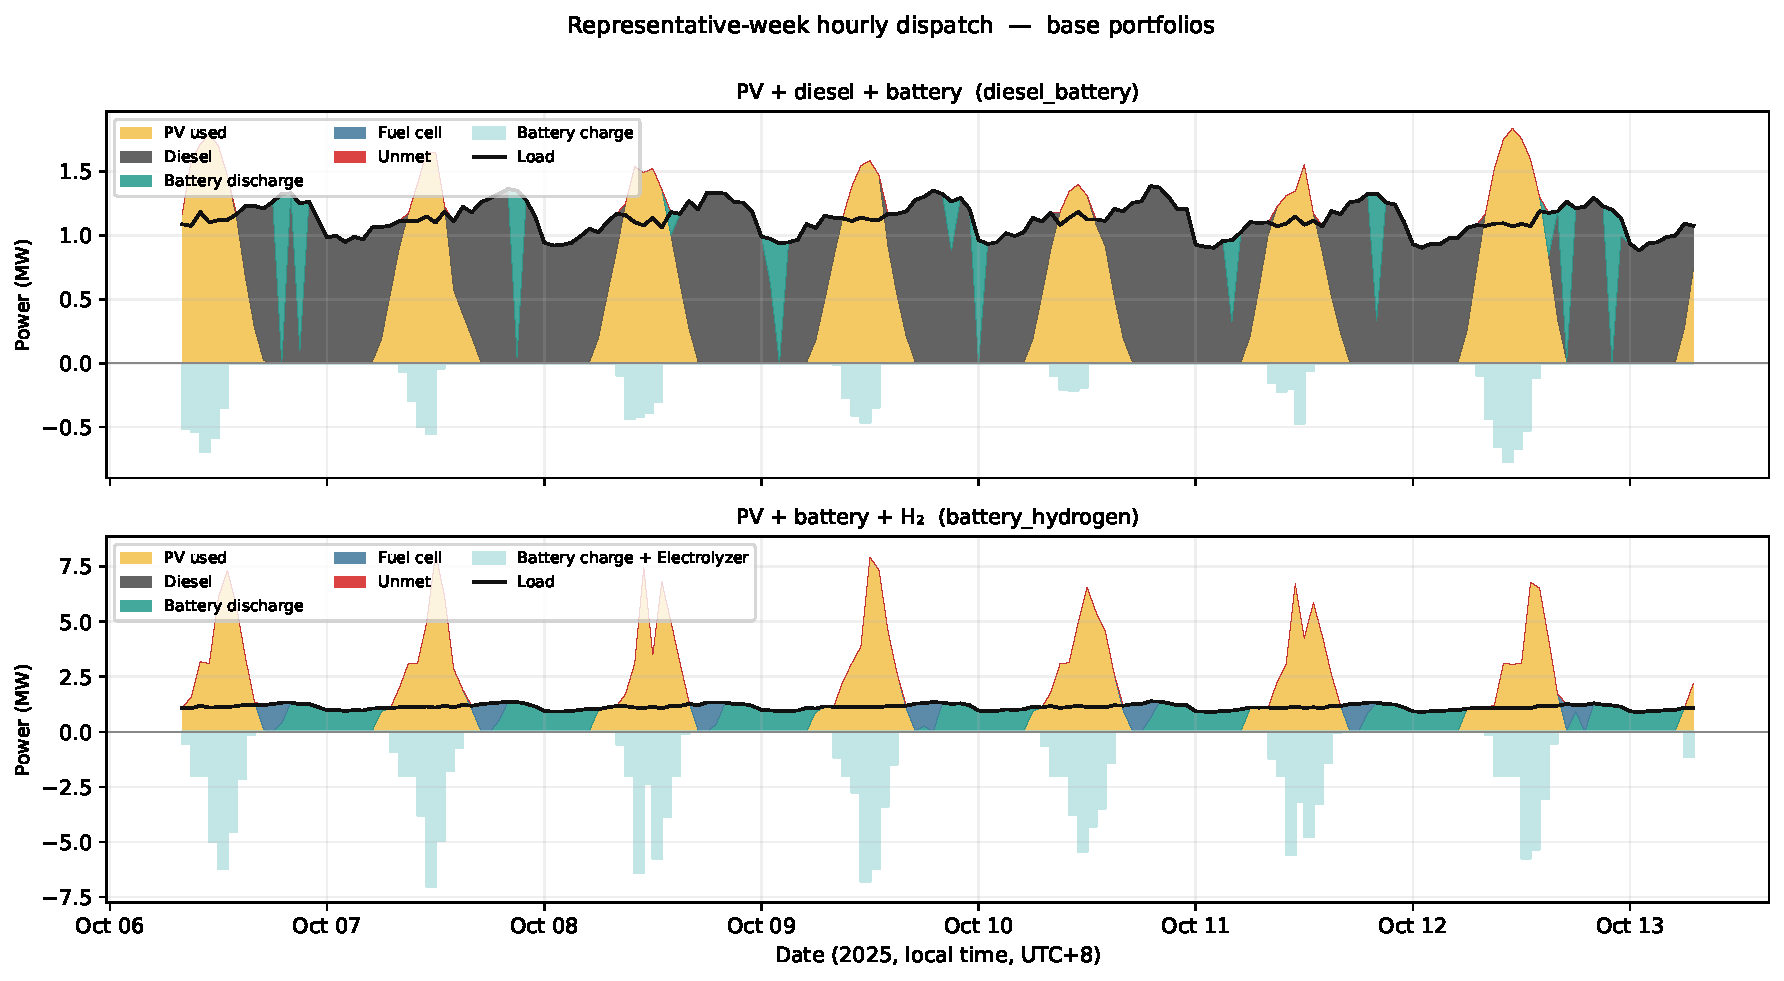
\includegraphics[width=\textwidth]{figures/fig02_base_dispatch.pdf}
\caption{Representative-week dispatch (week of 2025-10-06, in local time UTC+8) for
diesel-battery (top) and battery-hydrogen (bottom): daytime PV
charges the battery and electrolyser; the battery, and in low-PV periods the fuel
cell, serve the evening peak.}
\label{fig:dispatch}
\end{figure}

\subsection{Cost--resilience threshold}
\label{sub:thresh-res}
Figure~\ref{fig:threshold} maps the annual-cost difference between the two
portfolios across delivered diesel cost (100--1000~USD MWh$^{-1}$) and a
hydrogen-CAPEX multiplier (0.30--1.20), at the central carbon price of 150~USD
tCO$_2^{-1}$ and a 48-h outage. The zero-difference contour---the economic
crossover---passes through \textbf{378~USD MWh$^{-1}$} delivered diesel at the
baseline hydrogen CAPEX: below this the diesel-battery portfolio is
cheaper, above it battery-hydrogen is. This corresponds to roughly
3.8~USD L$^{-1}$, within the range reported for remote Philippine islands where
maritime fuel logistics dominate delivered cost. Reducing the hydrogen CAPEX to
0.30 of baseline lowers the crossover to 216~USD MWh$^{-1}$; raising it to 1.20
lifts it to 425~USD MWh$^{-1}$ (Table~\ref{tab:crossover}). Internalising the
resilience value of avoided unserved energy at $\mathrm{VOLL}=5000$~USD MWh$^{-1}$
lowers the crossover to \textbf{344~USD MWh$^{-1}$}, because the diesel portfolio's
residual outage exposure is then priced. The crossover is interior to the swept
diesel range for every multiplier level and reproduces, at the overlapping points,
the coarse three-value sensitivity of the original manuscript---now resolved as a
continuous frontier.

\begin{table}[H]
\centering
\caption{Economic and resilience-adjusted crossover diesel cost versus the
hydrogen-CAPEX multiplier $\mu$.}
\label{tab:crossover}
\resizebox{\textwidth}{!}{%
\begin{tabular}{lrr}
\toprule
$\mu$ (H$_2$ CAPEX) & Crossover, economic (USD/MWh) & Resilience-adjusted (USD/MWh) \\
\midrule
0.30 & 216 & 182 \\
1.00 & 378 & 344 \\
1.20 & 425 & 390 \\
\bottomrule
\end{tabular}%
}
\end{table}

\begin{figure}[H]
\centering
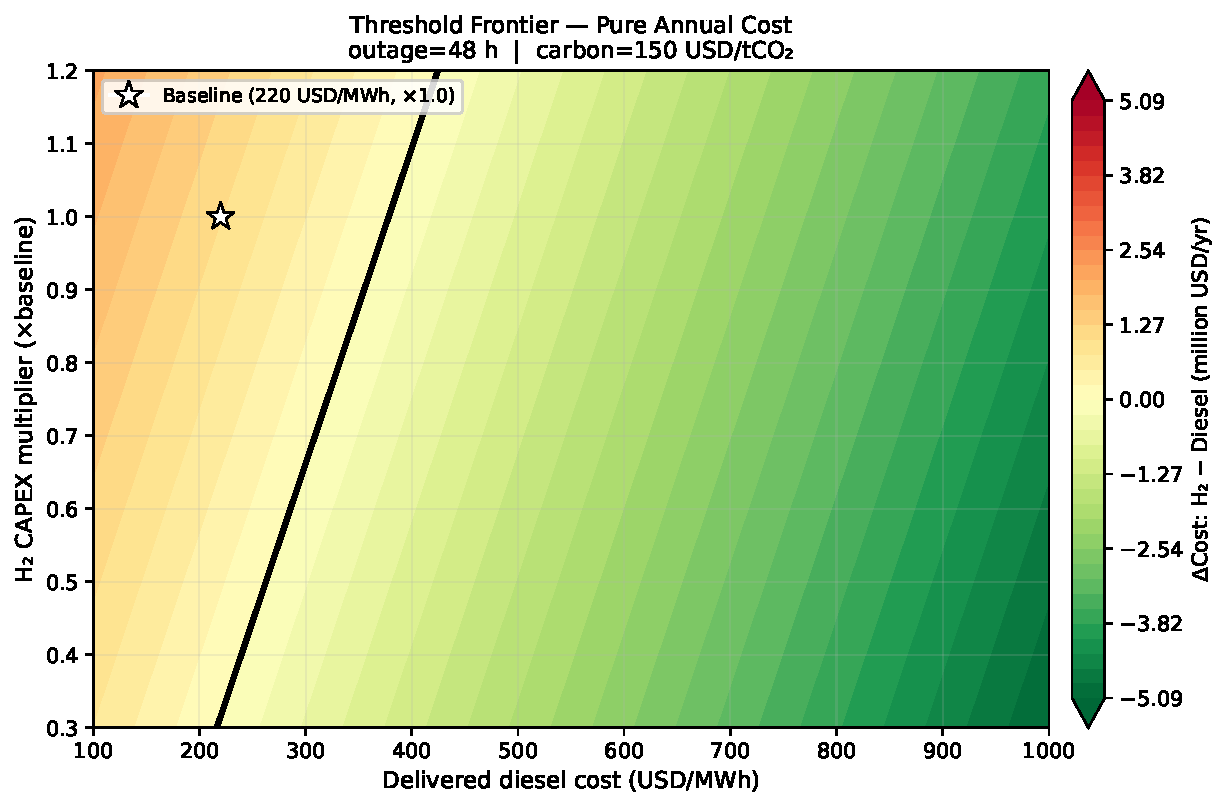
\includegraphics[width=\textwidth]{figures/fig03_threshold_contours.pdf}
\caption{Cost--resilience threshold: annual-cost difference
$\mathrm{AC}_{\mathrm{BH}}-\mathrm{AC}_{\mathrm{DB}}$ over delivered diesel cost and
hydrogen-CAPEX multiplier, at carbon 150~USD tCO$_2^{-1}$ and a 48-h outage. The
zero contour is the economic crossover (378~USD MWh$^{-1}$ at $\mu=1$). The
resilience-adjusted contour (VOLL 5000~USD MWh$^{-1}$) is shown in the
Supplementary (Fig.~S-fig03b).}
\label{fig:threshold}
\end{figure}

\subsection{What moves the frontier}
\label{sub:tornado-res}
Figure~\ref{fig:tornado} decomposes the crossover diesel cost into its sensitivity
to each design parameter, varied across its plausible range with the others held at
baseline (Table~\ref{tab:tornado}). The crossover is most sensitive by far to PV
capital cost (span 148~USD MWh$^{-1}$ across 0.6--1.2$\times$ of baseline), followed
by hydrogen-tank cost (92), electrolyser cost (66), and fuel-cell cost (45);
battery-energy cost contributes 11, and the electrolyser and fuel-cell efficiencies
move the crossover by less than 1~USD MWh$^{-1}$. The dominance of PV cost is
structural: the battery-hydrogen portfolio carries 14~MW of PV against the
diesel-battery portfolio's 2.8~MW, so a change in PV cost bears roughly
five-fold more strongly on the hydrogen side; normalised per unit fractional cost
change, PV is about 2.5$\times$ more influential than the hydrogen tank. The
near-zero efficiency sensitivities confirm that the hydrogen subsystem is sized by
energy balance and resilience, not by conversion efficiency. The actionable
implication is that PV-cost reduction---rather than electrolyser or fuel-cell
improvement---is the single most effective lever for hydrogen competitiveness.

\begin{table}[H]
\centering
\caption{Cost-driver sensitivity: span of the crossover diesel cost as each
parameter is varied across its plausible range.}
\label{tab:tornado}
\resizebox{\textwidth}{!}{%
\begin{tabular}{lr}
\toprule
Parameter (varied 0.6--1.2$\times$ baseline unless noted) & Crossover span (USD/MWh) \\
\midrule
PV capital cost          & 148.2 \\
Hydrogen-tank cost       & 91.9 \\
Electrolyser capital cost & 66.2 \\
Fuel-cell capital cost   & 45.3 \\
Battery-energy cost      & 11.0 \\
Fuel-cell efficiency     & 0.7 \\
Electrolyser efficiency  & 0.6 \\
\bottomrule
\end{tabular}%
}
\end{table}

\begin{figure}[H]
\centering
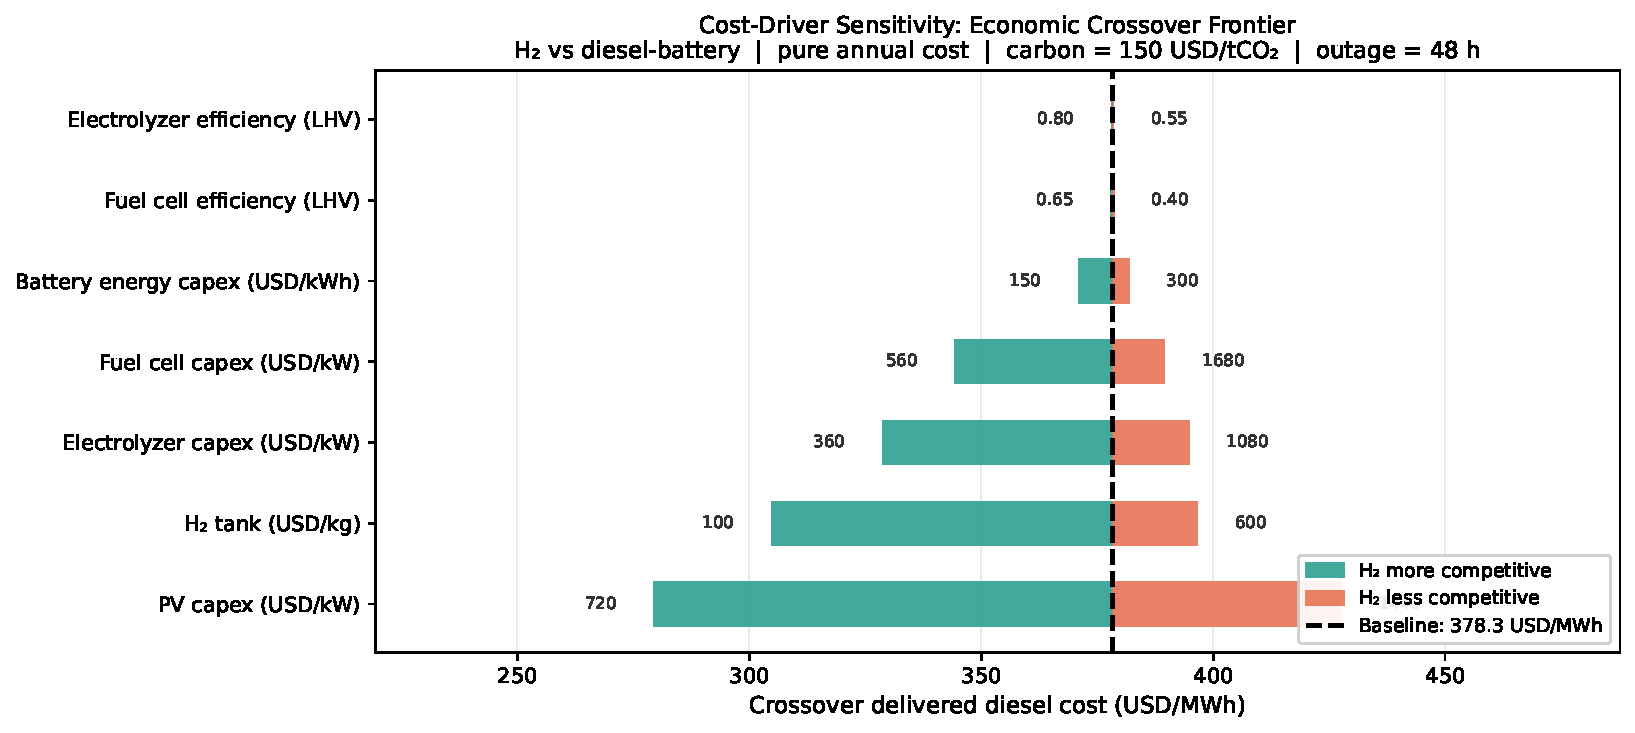
\includegraphics[width=0.85\textwidth]{figures/fig04_cost_driver_tornado.pdf}
\caption{Tornado of the crossover diesel cost: PV capital cost dominates, while
converter efficiencies are negligible.}
\label{fig:tornado}
\end{figure}

\subsection{Is the resilience advantage intrinsic? A matched-backbone test}
\label{sub:matched-res}
Section~\ref{sub:tornado-res} shows the frontier is dominated by PV cost, raising
the question of whether the hydrogen portfolio's advantages merely reflect its
larger PV--battery backbone. Figure~\ref{fig:matched} isolates the flexibility
technology by placing both portfolios on a common backbone---varying PV (7/10/14~MW)
and battery energy (8/12~MWh) identically (energy-to-power ratio 6~h) and retaining
only the distinguishing diesel or hydrogen subsystem (Table~\ref{tab:matched}). Two
results follow. First, the hydrogen portfolio requires a PV backbone of at least
14~MW to be viable at all: at 7--10~MW the electrolyser cannot be supplied enough
surplus to balance the 33.5\%-efficient hydrogen round-trip, the portfolio incurs
large unserved-energy penalties, and no crossover exists within the swept diesel
range. The large PV of the hydrogen design is thus a physical requirement, not
arbitrary oversizing. Second, and decisively, the resilience gap persists under a
matched backbone: at an identical 14~MW / 12~MWh backbone the diesel-battery
portfolio sheds critical load in the worst-case 48-h outage---its worst-case
survivable duration is zero hours and its worst-case CLSR is 0.98 across ten
seeds---while battery-hydrogen sustains the full 48 hours (CLSR 1.0), and the
diesel-battery worst-case survivability is zero at every backbone tested whereas
battery-hydrogen reaches full 48-h survivability once the PV backbone is large
enough to keep its store charged ($\ge$10~MW with the larger battery, and at
14~MW). Because the only difference at a matched
backbone is the flexibility subsystem, the resilience advantage is attributable to
the long-duration hydrogen store itself, not to fixed capacities.

Two points follow for interpretation. The matched-backbone economic crossover is
not the headline threshold: forcing the diesel-battery portfolio onto
hydrogen's 14~MW PV spine is not its cost-optimal configuration, so the matched
crossover (368~USD MWh$^{-1}$ at 14/8~MWh, 755 at 14/12~MWh) brackets rather than
replaces the 378~USD MWh$^{-1}$ obtained when each technology is compared at its own
appropriate scale. The matched backbone is therefore used to isolate the
\emph{resilience} contribution of the flexibility technology, not to redefine the
economic threshold; on the economic axis it confirms only that hydrogen's
competitiveness is sensitive to how much PV the comparison grants the diesel
alternative.

\begin{table}[H]
\centering
\caption{Matched-backbone comparison. Crossover ``---'' denotes none within the
swept diesel range (the hydrogen portfolio incurs large annual unserved-energy
penalties below 14~MW PV). CLSR$_{\min}$ and survivable hours are worst-case over
ten seeds for a 48-h outage with diesel unavailable.}
\label{tab:matched}
\resizebox{\textwidth}{!}{%
\begin{tabular}{llrrrr}
\toprule
Backbone & Crossover & \multicolumn{2}{c}{Diesel--battery} & \multicolumn{2}{c}{Battery--H$_2$} \\
(PV / battery) & (USD/MWh) & CLSR$_{\min}$ & surv.\ (h) & CLSR$_{\min}$ & surv.\ (h) \\
\midrule
7 MW / 8 MWh       & ---   & 0.88 & 0 & 0.98 & 9  \\
10 MW / 12 MWh     & ---   & 0.96 & 0 & 1.00 & 48 \\
14 MW / 8 MWh      & 368   & 0.92 & 0 & 1.00 & 48 \\
14 MW / 12 MWh     & 755   & 0.98 & 0 & 1.00 & 48 \\
\bottomrule
\end{tabular}%
}
\end{table}

\begin{figure}[H]
\centering
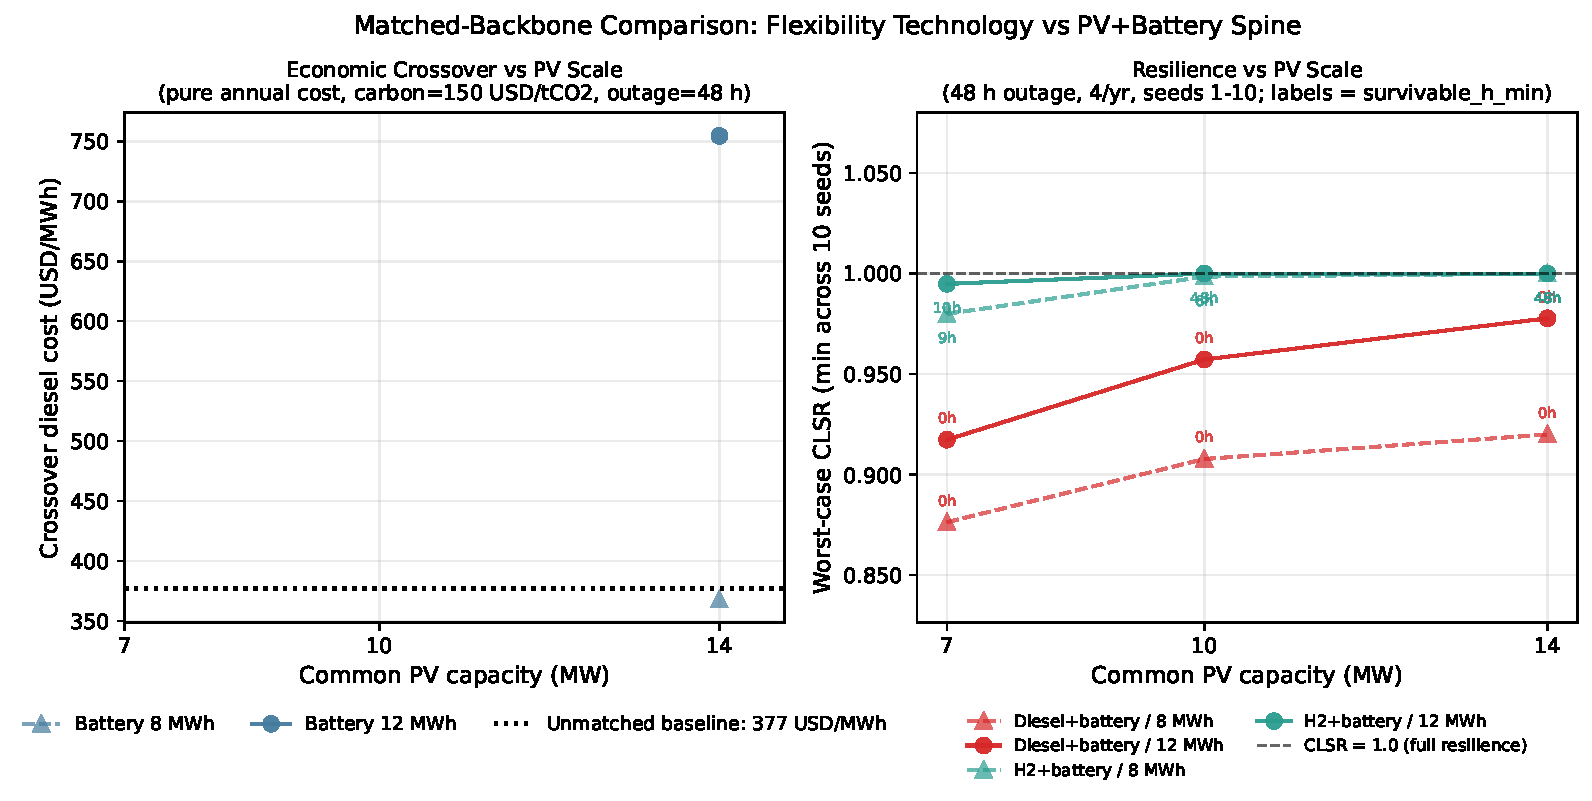
\includegraphics[width=\textwidth]{figures/fig05_matched_backbone.pdf}
\caption{Matched-backbone comparison across common PV and battery sizes:
battery-hydrogen requires $\ge$14~MW PV to be feasible, and at a matched
backbone retains full 48-h survivability while diesel-battery sheds critical
load (worst-case survivable duration 0~h).}
\label{fig:matched}
\end{figure}

\subsection{Robustness to the diesel-support assumption}
\label{sub:robust-res}
The resilience comparison so far assumes diesel is unavailable during an outage.
Figure~\ref{fig:robust} relaxes this across graded support cases. Under full
unavailability (D0) the diesel-battery worst-case survivability is zero
hours and the worst-case CLSR is 0.58 across ten seeds---the single-seed value of
0.65 in the original manuscript was optimistic. Restoring support closes the gap
only above clear thresholds: the diesel-battery portfolio matches the
hydrogen portfolio's 48-h survivability only with $\ge$50\% derating (D1) or
$\ge$12~h of fuel (D2). Most strikingly, any start-up or delivery delay collapses
worst-case survivability to zero---even a six-hour delay (D3)---because the battery
depletes before diesel arrives during the worst-timed outage. With diesel fully
available but its delivered fuel cost shocked (D4), the economic crossover is
unchanged at 378~USD MWh$^{-1}$; above roughly 380~USD MWh$^{-1}$ the
battery-hydrogen portfolio is simultaneously cheaper and at least as
resilient. The hydrogen portfolio's value is therefore specifically a hedge against
degradation of diesel support---derating, fuel limits, or delivery delay---the
characteristic failure modes during storms and logistics disruptions.

\begin{figure}[H]
\centering
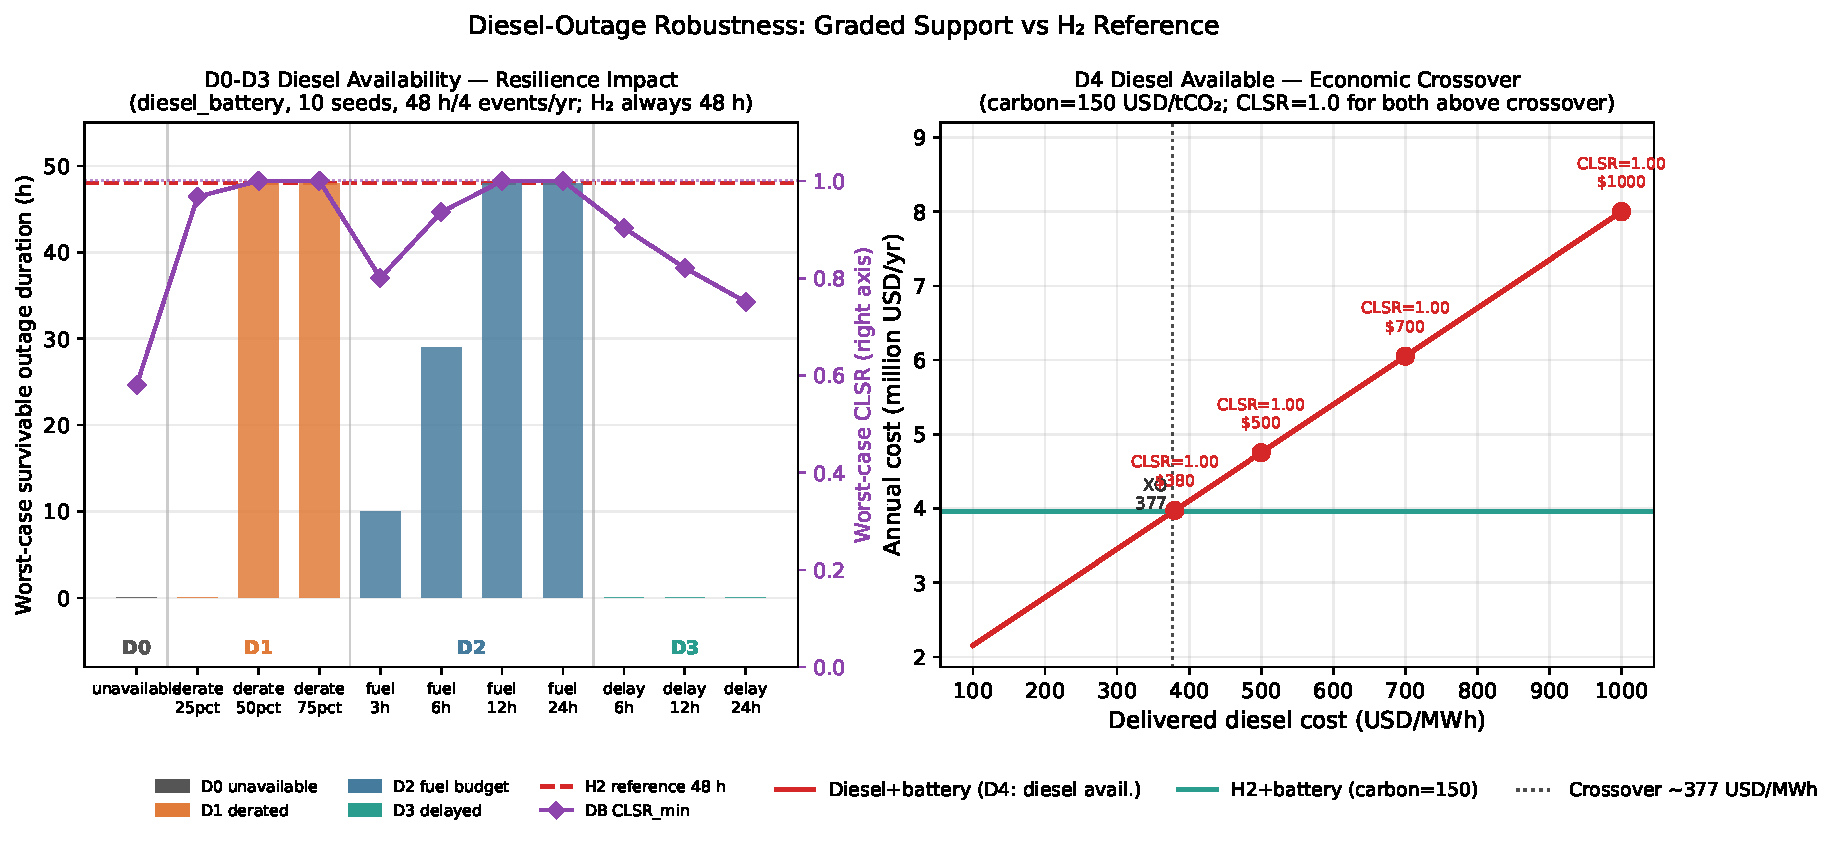
\includegraphics[width=\textwidth]{figures/fig06_outage_robustness.pdf}
\caption{Graded diesel-support robustness. Worst-case survivability of
diesel-battery reaches the hydrogen reference (48~h) only with
$\ge$50\% derating (D1) or $\ge$12~h fuel (D2); any delay (D3) returns it to zero.
battery-hydrogen is the invariant reference.}
\label{fig:robust}
\end{figure}

\subsection{Dynamic feasibility}
\label{sub:freq-res}
Figure~\ref{fig:freq} screens primary-frequency response (Table~\ref{tab:freq}).
Under a 10\% load step all three portfolios hold the frequency nadir above 49.0~Hz;
the RoCoF is 0.86~Hz s$^{-1}$ for diesel-battery (within both islanded and
mainland limits, owing to synchronous-generator inertia), 1.88~Hz s$^{-1}$ for
battery-only, and 2.06~Hz s$^{-1}$ for battery-hydrogen---the
last marginally above the 2.0~Hz s$^{-1}$ islanded screening value, which a modest
increase of the grid-forming virtual-inertia constant to $\ge 1.2$~s removes. The
portfolios diverge sharply only in the contingency that matters most: loss of the
diesel generator. When the 1.65~MW diesel trips and the 1.5~MW battery must assume
grid-forming, the instantaneous RoCoF reaches 27~Hz s$^{-1}$ (5.9~Hz s$^{-1}$ over
the relay-relevant 500~ms window) and the nadir falls to 45.9~Hz, because the
battery is undersized relative to the generation it must instantly replace; full
rebalancing requires under-frequency load shedding, though the battery alone
sustains the 0.55 critical fraction (1.5~MW $\ge$ 0.91~MW). The
diesel-battery portfolio is thus dynamically weakest during exactly the
event---diesel loss---at which Sections~\ref{sub:matched-res}--\ref{sub:robust-res}
found it energetically weakest, whereas battery-hydrogen, with a larger
grid-forming battery, fuel-cell droop support, and no diesel to lose, avoids the
contingency. The dynamic screen reinforces rather than qualifies the cost--resilience
conclusion.

\begin{table}[H]
\centering
\small
\caption{Primary-frequency screening metrics. Screening limits: nadir
$\ge 49.0$~Hz, $|\mathrm{RoCoF}|<2.0$~Hz s$^{-1}$ (islanded).}
\label{tab:freq}
\begin{tabularx}{\textwidth}{llrrX}
\toprule
Disturbance & Portfolio & Nadir (Hz) & RoCoF (Hz/s) & Note \\
\midrule
10\% load step & diesel-battery   & $>$49 & 0.86 & pass \\
10\% load step & battery-only     & $>$49 & 1.88 & pass \\
10\% load step & battery-hydrogen & $>$49 & 2.06 & marginal (VSM tuning) \\
Diesel trip    & diesel-battery   & 45.9  & 27.5 & 5.9 Hz/s at 500\,ms; UFLS, critical load held \\
\bottomrule
\end{tabularx}
\end{table}

\begin{figure}[H]
\centering
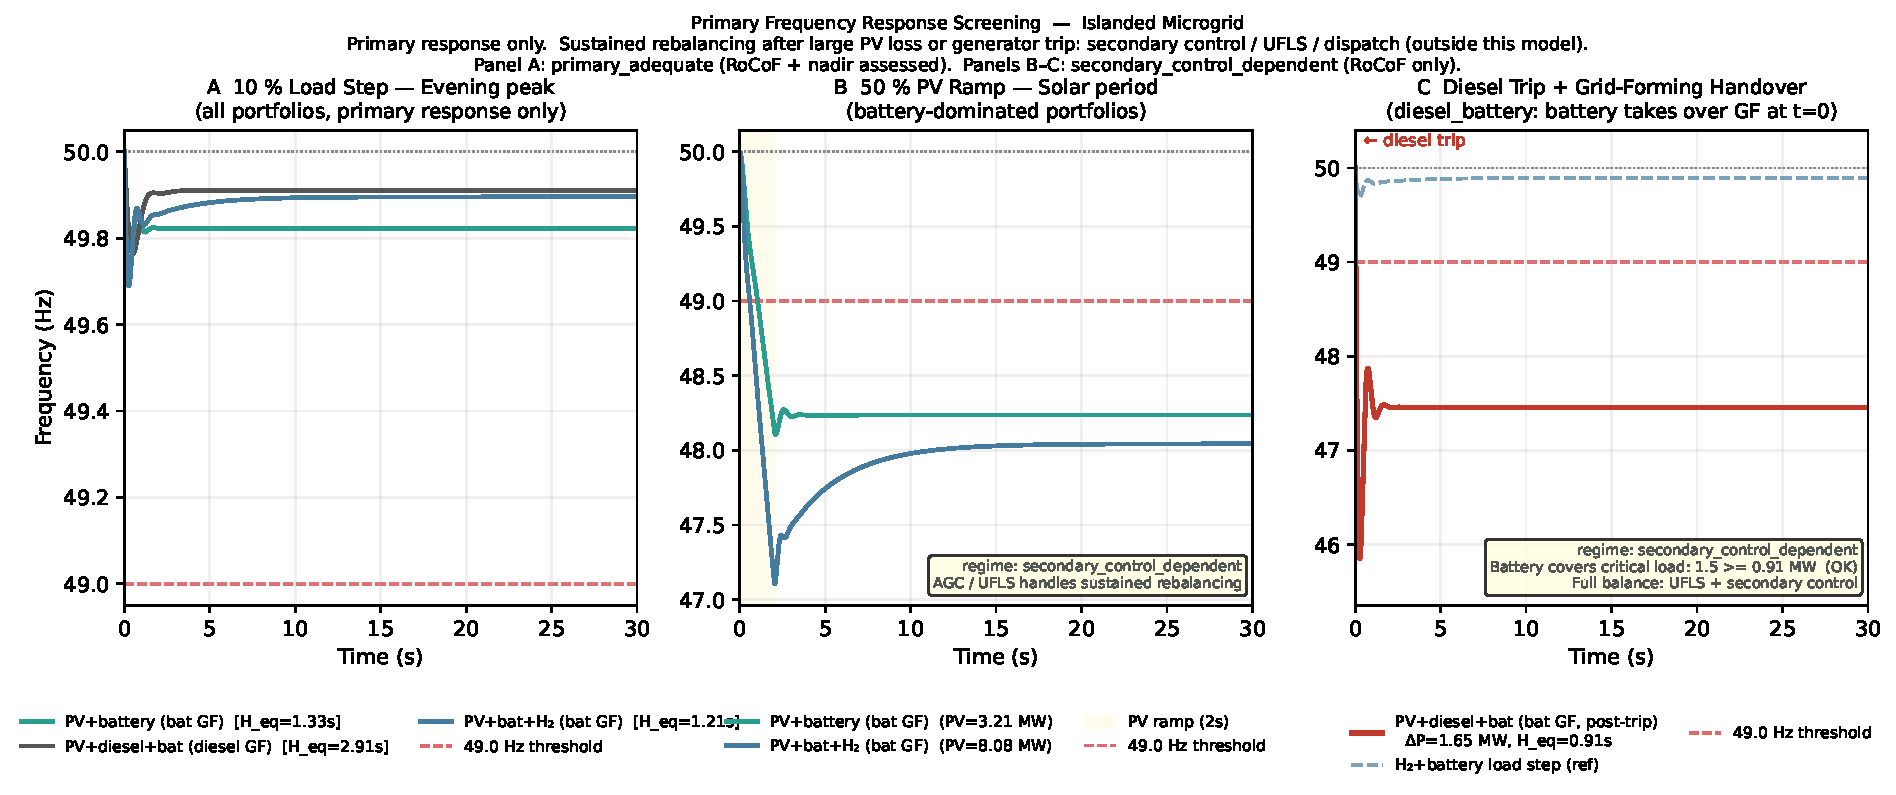
\includegraphics[width=\textwidth]{figures/fig07_frequency_response.pdf}
\caption{Reduced-order primary-frequency response. Load step (left): all
portfolios hold nadir $>$49~Hz. Diesel trip (right): diesel-battery
exhibits a deep nadir and high RoCoF during the grid-forming hand-over.}
\label{fig:freq}
\end{figure}

\subsection{Synthesis}
\label{sub:synth}
Taken together (Figs.~\ref{fig:threshold}--\ref{fig:freq}), the battery--hydrogen
portfolio is the defensible design under either of two independently realistic
conditions: a delivered diesel cost at or above 378~USD MWh$^{-1}$
(Sections~\ref{sub:thresh-res}, \ref{sub:robust-res}), or any material degradation
of diesel support during outages (Section~\ref{sub:robust-res}), under which the
diesel--battery worst-case survivability collapses---in both energy
(Sections~\ref{sub:matched-res}--\ref{sub:robust-res}) and frequency-dynamic
(Section~\ref{sub:freq-res}) terms---while the hydrogen store holds full
critical-load service. Both conditions characterise remote-island and typhoon
contingencies. The hydrogen design's large PV is a physical requirement of the
round-trip (Section~\ref{sub:matched-res}), and PV-cost reduction is the most
powerful lever on its competitiveness (Section~\ref{sub:tornado-res}).

%=====================================================================
\section{Discussion}
\label{sec:disc}

\subsection{Principal findings}
The analysis yields a single, design-actionable picture rather than the qualitative
claim that hydrogen becomes attractive when diesel is expensive. The economic
crossover between the two portfolios is a continuous frontier whose central value is
378~USD MWh$^{-1}$ of delivered diesel at baseline hydrogen cost and a
150~USD tCO$_2^{-1}$ carbon price, falling to 344~USD MWh$^{-1}$ once the resilience
value of avoided unserved energy is internalised, and ranging from 216 to
425~USD MWh$^{-1}$ as hydrogen capital varies over 0.30--1.20$\times$. The position
of that frontier is governed overwhelmingly by PV capital cost---2.5 times more
strongly than by hydrogen-tank cost and two orders of magnitude more strongly than
by converter efficiency---because the hydrogen portfolio is intrinsically
PV-intensive (14 versus 2.8~MW) to balance a 33.5\%-efficient round-trip. The
resilience advantage is not an artefact of the larger backbone: on an identical
PV--battery backbone the diesel--battery portfolio sheds critical load in a
worst-case 48-h outage (zero guaranteed survivable hours, worst-case CLSR 0.98)
while the hydrogen portfolio sustains the full duration, so
the advantage is attributable to the long-duration store itself. That advantage is
conditional on the diesel-unavailability assumption; relaxing it shows the diesel
portfolio matches hydrogen only above clear support thresholds ($\ge$50\% derate or
$\ge$12~h fuel) and that any start-up delay---even six hours---collapses its
worst-case survivability. Finally, the diesel portfolio is dynamically weakest at
precisely the diesel-trip contingency where it is energetically weakest, with a
500~ms RoCoF of 5.9~Hz s$^{-1}$ and a 45.9~Hz nadir requiring load shedding, whereas
the hydrogen portfolio has no equivalent single-point contingency.

\subsection{Why the result is not self-evident}
That hydrogen wins when diesel is dear is, taken alone, unsurprising. The
contribution here is the structure behind that statement, which is neither obvious a
priori nor recoverable from a coarse break-even calculation. First, the crossover is
set not by the hydrogen chain's own cost or efficiency but by PV capital
cost---a consequence of the portfolio's energy balance that only a full 8760-h
optimisation reveals, and one that redirects cost-reduction effort from converters
toward PV. Second, the resilience gap survives a matched backbone: a reader could
reasonably attribute hydrogen's outage performance to its larger PV and battery, and
the matched-backbone experiment is required to show that it does not. Third, the
diesel portfolio's resilience is far more fragile than a single-seed or
perfect-availability analysis implies; the finding that a six-hour diesel-start
delay erases worst-case survivability entirely, while a 50\% derate or a 12-h fuel
limit does not, is a non-monotone, operationally specific result. Fourth, the most
dangerous frequency event for the diesel portfolio is the loss of the very asset
that provides its inertia, so that the technology improving small-signal RoCoF also
creates the binding large-disturbance contingency. Each is a design-actionable,
non-obvious refinement of the headline.

\subsection{Relation to prior work}
The individual techniques used here are established; the contribution is their
integration and the attribution it enables. Prior island studies optimise component
sizing with tools such as HOMER and mixed-integer programs
\cite{pascasio_2021_philippines_pv_wind,castro_2024_208_islands_transition}, and
recent work has tested fuel-constrained or graded-availability outages
\cite{marqusee2021resilience,sharifpour_2023_hydrogen_extreme_events} and combined
techno-economic with dynamic assessment
\cite{huang_2023_economic_resilient_h2_microgrid,shahbazbegian_2023_resilience_p2h}.
What has been missing is a single framework that (i) resolves the cost--resilience
trade-off as a continuous, carbon-priced threshold rather than a point estimate,
(ii) attributes that threshold to specific design parameters, (iii) isolates the
contribution of the flexibility technology from that of the shared backbone, and
(iv) verifies dynamic feasibility for the same portfolios and contingencies. The
matched-backbone experiment (Section~\ref{sub:matched-res}) is the methodological
centrepiece: by holding the PV--battery spine fixed it separates the effect of the
long-duration store from that of capacity, which sizing-only optimisations cannot do.
Relative to survivability-focused resilience studies
\cite{marqusee2021resilience,gao_2016_critical_load_restoration,mishra2023microgrid},
the present work links the survivability metric to the economic threshold and to a
primary-frequency screen on the same system; relative to integrated
techno-economic--dynamic studies, it adds the attribution and technology-isolation
analyses and grounds the comparison in a real measured-weather year for a
representative Philippine off-grid context
\cite{castro_2022_634_islands_hres,meschede2019transferability}. The Philippine
setting is not incidental: with several hundred NPC-SPUG diesel islands and
operational PV--battery--diesel microgrids, delivered diesel costs and outage
exposure of the magnitude examined here are realistic rather than hypothetical
\cite{ocon_bertheau_2019_philippines_diesel_pvbatt,bertheau2018resilient}.

\subsection{Limitations and future work}
Several limitations bound the claims and define the next steps. The dispatch uses a
single measured weather year (2025) at one grid cell; interannual variability and a
typhoon-year stress test are not captured and would refine both the cost and the
resilience estimates. The demand is a representative calibrated archetype rather
than metered island load, because public hourly demand for individual off-grid
islands is scarce; substituting a metered profile would sharpen the demand-side
detail without altering the structure of the comparison. The operational model is a
deterministic linear program with perfect foresight, which yields a lower bound on
operating cost; rolling-horizon or stochastic operation would test the robustness of
the cost figures, although the resilience results derive from a separate,
foresight-free outage simulation. The frequency analysis is a reduced-order
primary-response screen; it establishes feasibility and ranks contingencies but is
not a substitute for electromagnetic-transient simulation, secondary/automatic
generation control, under-frequency load-shedding design, or protection
coordination, which are needed before deployment and which the marginal
battery-hydrogen RoCoF and the diesel-trip nadir both motivate. The system
is a single island with PV as the only renewable resource; wind hybridisation,
inter-island interconnection, and component degradation are left to future work.
Finally, hydrogen costs are evolving rapidly; the capital-multiplier sweep partially
internalises this, but the crossover should be re-evaluated as cost data mature.

Two further caveats sharpen these points. First, outage start times are sampled
uniformly across the year rather than correlated with the adverse-weather
episodes---multi-day typhoon overcast---that most stress an islanded system;
although the worst-case-over-seeds statistic captures low-irradiance onsets,
explicitly conditioning outages on a typhoon-affected weather year would be a more
demanding and realistic resilience test. Second, the flexibility components
(electrolyser, fuel cell, tank, and diesel rating) are held at representative fixed
sizes; co-optimising these alongside the PV--battery backbone would refine the
absolute thresholds, though the matched-backbone design already controls for the
dominant PV--battery sizing effect.

%=====================================================================
\section{Conclusion}
\label{sec:concl}

For islanded power systems, the choice between a PV--diesel--battery and a
PV--battery--hydrogen portfolio is governed by a quantifiable cost--resilience
threshold rather than a qualitative preference. Using an 8760-h cost-optimal
dispatch model driven by real NASA POWER weather for a representative Philippine
off-grid island, together with a worst-case outage simulation and a reduced-order
frequency screen, we find that the battery--hydrogen portfolio is the defensible
design under either of two independently realistic conditions: a delivered diesel
cost at or above 378~USD MWh$^{-1}$ (344~USD MWh$^{-1}$ when avoided unserved energy
is valued), or any material degradation of diesel support during outages---a derate
below 50\%, a fuel budget under 12 hours, or any start-up delay---each of which
collapses the diesel portfolio's worst-case survivability to near zero in both
energy and frequency-dynamic terms while the hydrogen store sustains full
critical-load service for 48 hours. The threshold's position is set principally by
PV capital cost, making PV-cost reduction the most effective lever on hydrogen
competitiveness, while converter efficiency is nearly immaterial; and a
matched-backbone test shows the resilience advantage to be intrinsic to the
long-duration hydrogen store rather than a by-product of the larger backbone the
store requires. These conditions correspond to exactly the remote-island and storm
contingencies that motivate off-grid hydrogen, converting a qualitative intuition
into design-actionable thresholds, attributions, and feasibility checks that island
planners can apply directly.

%=====================================================================
\section*{Data availability}
All code, model configuration, input data (real NASA POWER 2025 weather and the
calibrated load profile), and the scripts that generate every figure and table are
openly available at \url{https://github.com/exoprime-sketch/microgrid-h2-paper} and
archived at Zenodo (DOI 10.5281/zenodo.19658561).

\section*{Declaration of competing interest}
The author declares that he has no known competing financial interests or personal
relationships that could have appeared to influence the work reported in this paper.

\section*{Funding}
This research did not receive any specific grant from funding agencies in the
public, commercial, or not-for-profit sectors. % EDIT if a funder applies.

\section*{Declaration of generative AI and AI-assisted technologies}
During the preparation of this work the author used AI-assisted tools for language editing.

\bibliographystyle{elsarticle-num}
\bibliography{refs,refs_additions}

\end{document}
